\documentclass[a4paper]{article}
\usepackage[pdftex]{graphicx}
\usepackage[utf8]{inputenc}
\usepackage{enumerate}
\usepackage{icomma}
\usepackage{siunitx}
\sisetup{locale=DE} 
\usepackage{amssymb}
\usepackage{tikz}
\usepackage{href-ul}
\hypersetup{
	colorlinks=true,
	linkcolor=blue,
	urlcolor=blue}
\usepackage{geometry}
\geometry{a4paper, top=15mm, left=15mm, right=15mm, bottom=15mm,
	headsep=10mm, footskip=12mm}

\begin{document}
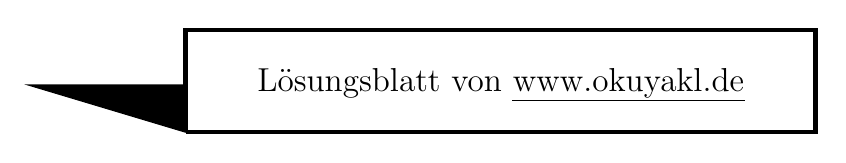
\begin{tikzpicture}(10,3)
	\draw[ultra thick](2,0) --(10,0) -- (10,1.3) --(2,1.3) -- (2,0);
	\draw[fill=black](2,0)-- (0,.6) -- (2,.6) -- (2,0);
	\node at (6,.6) {\large Lösungsblatt von \href{https://www.okuyakl.de}{www.okuyakl.de}};
\end{tikzpicture}
\vspace{0.5 cm}
\noindent {\bf Aufgabe 1. a)}\\
Die Volumenformel für dieses Prisma lösen wir nach $e$ auf:
$$
\renewcommand{\arraystretch}{2}
\begin{array}{rcll}
 V &=& G \cdot h \\
 V &=& {1 \over 2} e \cdot f \cdot h &|:f \quad |:h \quad |\cdot 2\\
 {2 V \over f \cdot h} &=& e 
\end{array}
$$

\noindent {\bf Aufgabe 1. b)}\\
Wir setzen die gegebenen Werte ein:
$${ 2 \cdot 25,5 \over 4,3 \cdot 6,6} = \SI{1,80}{\centi\meter}$$

\noindent {\bf Aufgabe 2.}\\
Wir gehen schrittweise vor. Zuerst berechnen wir die Sechseckfläche. Sie besteht aus sechs gleichseitigen Dreiecken der Seitenlänge $\SI{6}{\centi\meter}$. Dann ist die Fläche eines Dreiecks: 
$$A_D={1\over 2} \cdot a \cdot b \cdot \sin\gamma = {1\over 2}\cdot 6^2 \cdot \sin 60^\circ = 9\sqrt{3} =\SI{15,59}{\centi\meter^2}$$
Das Volumen des sechseckigen Prismas ist dann:
$$V_{Pr}=6\cdot A_D \cdot h = 6 \cdot 9 \cdot \sqrt{3} \cdot 23 = \SI{2151,21}{\centi\meter^3}$$
Das Volumen des vollen Glaszylinders ist:
$$V_{Z}=\pi r^2 \cdot h = \pi \cdot 7^2 \cdot 23 =\SI{3540,57}{\centi\meter}^3$$
Das Gewicht des Restkörpers ist die Differenz von Zylinder und Prisma multipliziert mit der Dichte:
$$ m = (3540,57-2151,21)\SI{}{\centi\meter^3} \cdot \SI{2,4}{\gram\per\centi\meter^3}=\SI{3334,47}{\gram}=\SI{3,33}{\kilogram}$$
 
\noindent{\bf Aufgabe 3. a)}\\
Mit dem Satz des Pythagoras berechnen wir:
$$
\renewcommand{\arraystretch}{2}
\begin{array}{rcll}
\left({a\over 2}\right)^2 + h_k^2 & = & h_a^2 & | - h_k^2 \\
\left({a\over 2}\right)^2 & = & h_a^2 - h_k^2 &| \sqrt{\qquad}\\
{a\over 2} & = & \sqrt{h_a^2 - h_k^2} &|\cdot 2 \\
a & = & 2 \cdot \sqrt{(\SI{9,4}{\centi\meter})^2-(\SI{7,8}{\centi\meter})^2} & = \SI{10,5}{\centi\meter}   
\end{array}
$$
Die Seitenkante berechnet sich mit:
$$
\renewcommand{\arraystretch}{2}
\begin{array}{rcll}
s^2 & = & \left({a\over 2}\right)^2 + h_a^2 & | \sqrt{\qquad} \\
s & = & \sqrt{(\SI{5,25}{\centi\meter})^2 + (\SI{9,4}{\centi\meter})^2} & =\SI{10,77}{\centi\meter}
\end{array}
$$
Für das Pyramidenvolumen erhalten wir:
$$V={1\over 3} \cdot a^2 \cdot h_k= {1\over 3} \cdot  (\SI{10,5}{\centi\meter})^2 \cdot \SI{7,8}{\centi\meter} = \SI{286,7}{\centi\meter^3}$$
Die Mantelfläche besteht aus vier gleichschenkligen Dreiecken:
$$M=4\cdot {1\over 2} a \cdot h_a= 2\cdot \SI{10,5}{\centi\meter} \cdot \SI{9,4}{\centi\meter} = \SI{197,4}{\centi\meter^2}$$
Um die gesamte Oberfläche zu erhalten, addieren wir hierzu noch die Grundfläche:
$$O = M + a^2 = \SI{197,4}{\centi\meter^2}+(\SI{10,5}{\centi\meter})^2 = \SI{307,7}{\centi\meter^2}$$ 

\noindent{\bf Aufgabe 3. b)}\\
Wir verwenden wieder den Satz des Pythagoras:
$$
\renewcommand{\arraystretch}{2}
\begin{array}{rcll}
h_k^2 + \left({a\over 2}\right)^2 & = & h_a^2 &| -\left({a\over 2}\right)^2 \\
h_k^2 & = & h_a^2 - \left({a\over 2}\right)^2 & | \sqrt{\qquad}\\
h_k & = & \sqrt{(\SI{18}{\centi\meter})^2 - (\SI{7,5}{\centi\meter})^2} & = \SI{16,4}{\centi\meter}\\
\end{array}
$$
Für die Seitenkante $s$ gilt:
$$s=\sqrt{\left({a\over 2}\right)^2 + h_a^2}= \sqrt{(\SI{7,5}{\centi\meter})^2 + (\SI{18}{\centi\meter})^2 } = \SI{19,5}{\centi\meter}$$
Das Volumen berechnen wir mit:
$$V={1\over 3} \cdot a^2 \cdot h_k= {1\over 3} \cdot  (\SI{15}{\centi\meter})^2 \cdot \SI{16,4}{\centi\meter} = \SI{1230}{\centi\meter^3}$$
Die Mantelfläche besteht aus vier gleichschenkligen Dreiecken:
$$M=4\cdot {1\over 2} a \cdot h_a= 2\cdot \SI{15}{\centi\meter} \cdot \SI{18}{\centi\meter} = \SI{540}{\centi\meter^2}$$
Um die gesamte Oberfläche zu erhalten, addieren wir hierzu noch die Grundfläche:
$$O = M + a^2 = \SI{540}{\centi\meter^2}+(\SI{15}{\centi\meter})^2 = \SI{765}{\centi\meter^2}$$ 

\begin{center}
	\includegraphics[width=7 cm]{../../viecher/endcomic.pdf}
	
	Hier geht es zurück zum \href{https://www.okuyakl.de/math/m9korL046/aa046.pdf}{Aufgabenblatt}
\end{center}


\end{document}

